\vspace{-1.5ex}
\section{Method}
\label{sec:method}
\vspace{-0.5ex}

% \begin{figure*}[!t]
% \centering
%   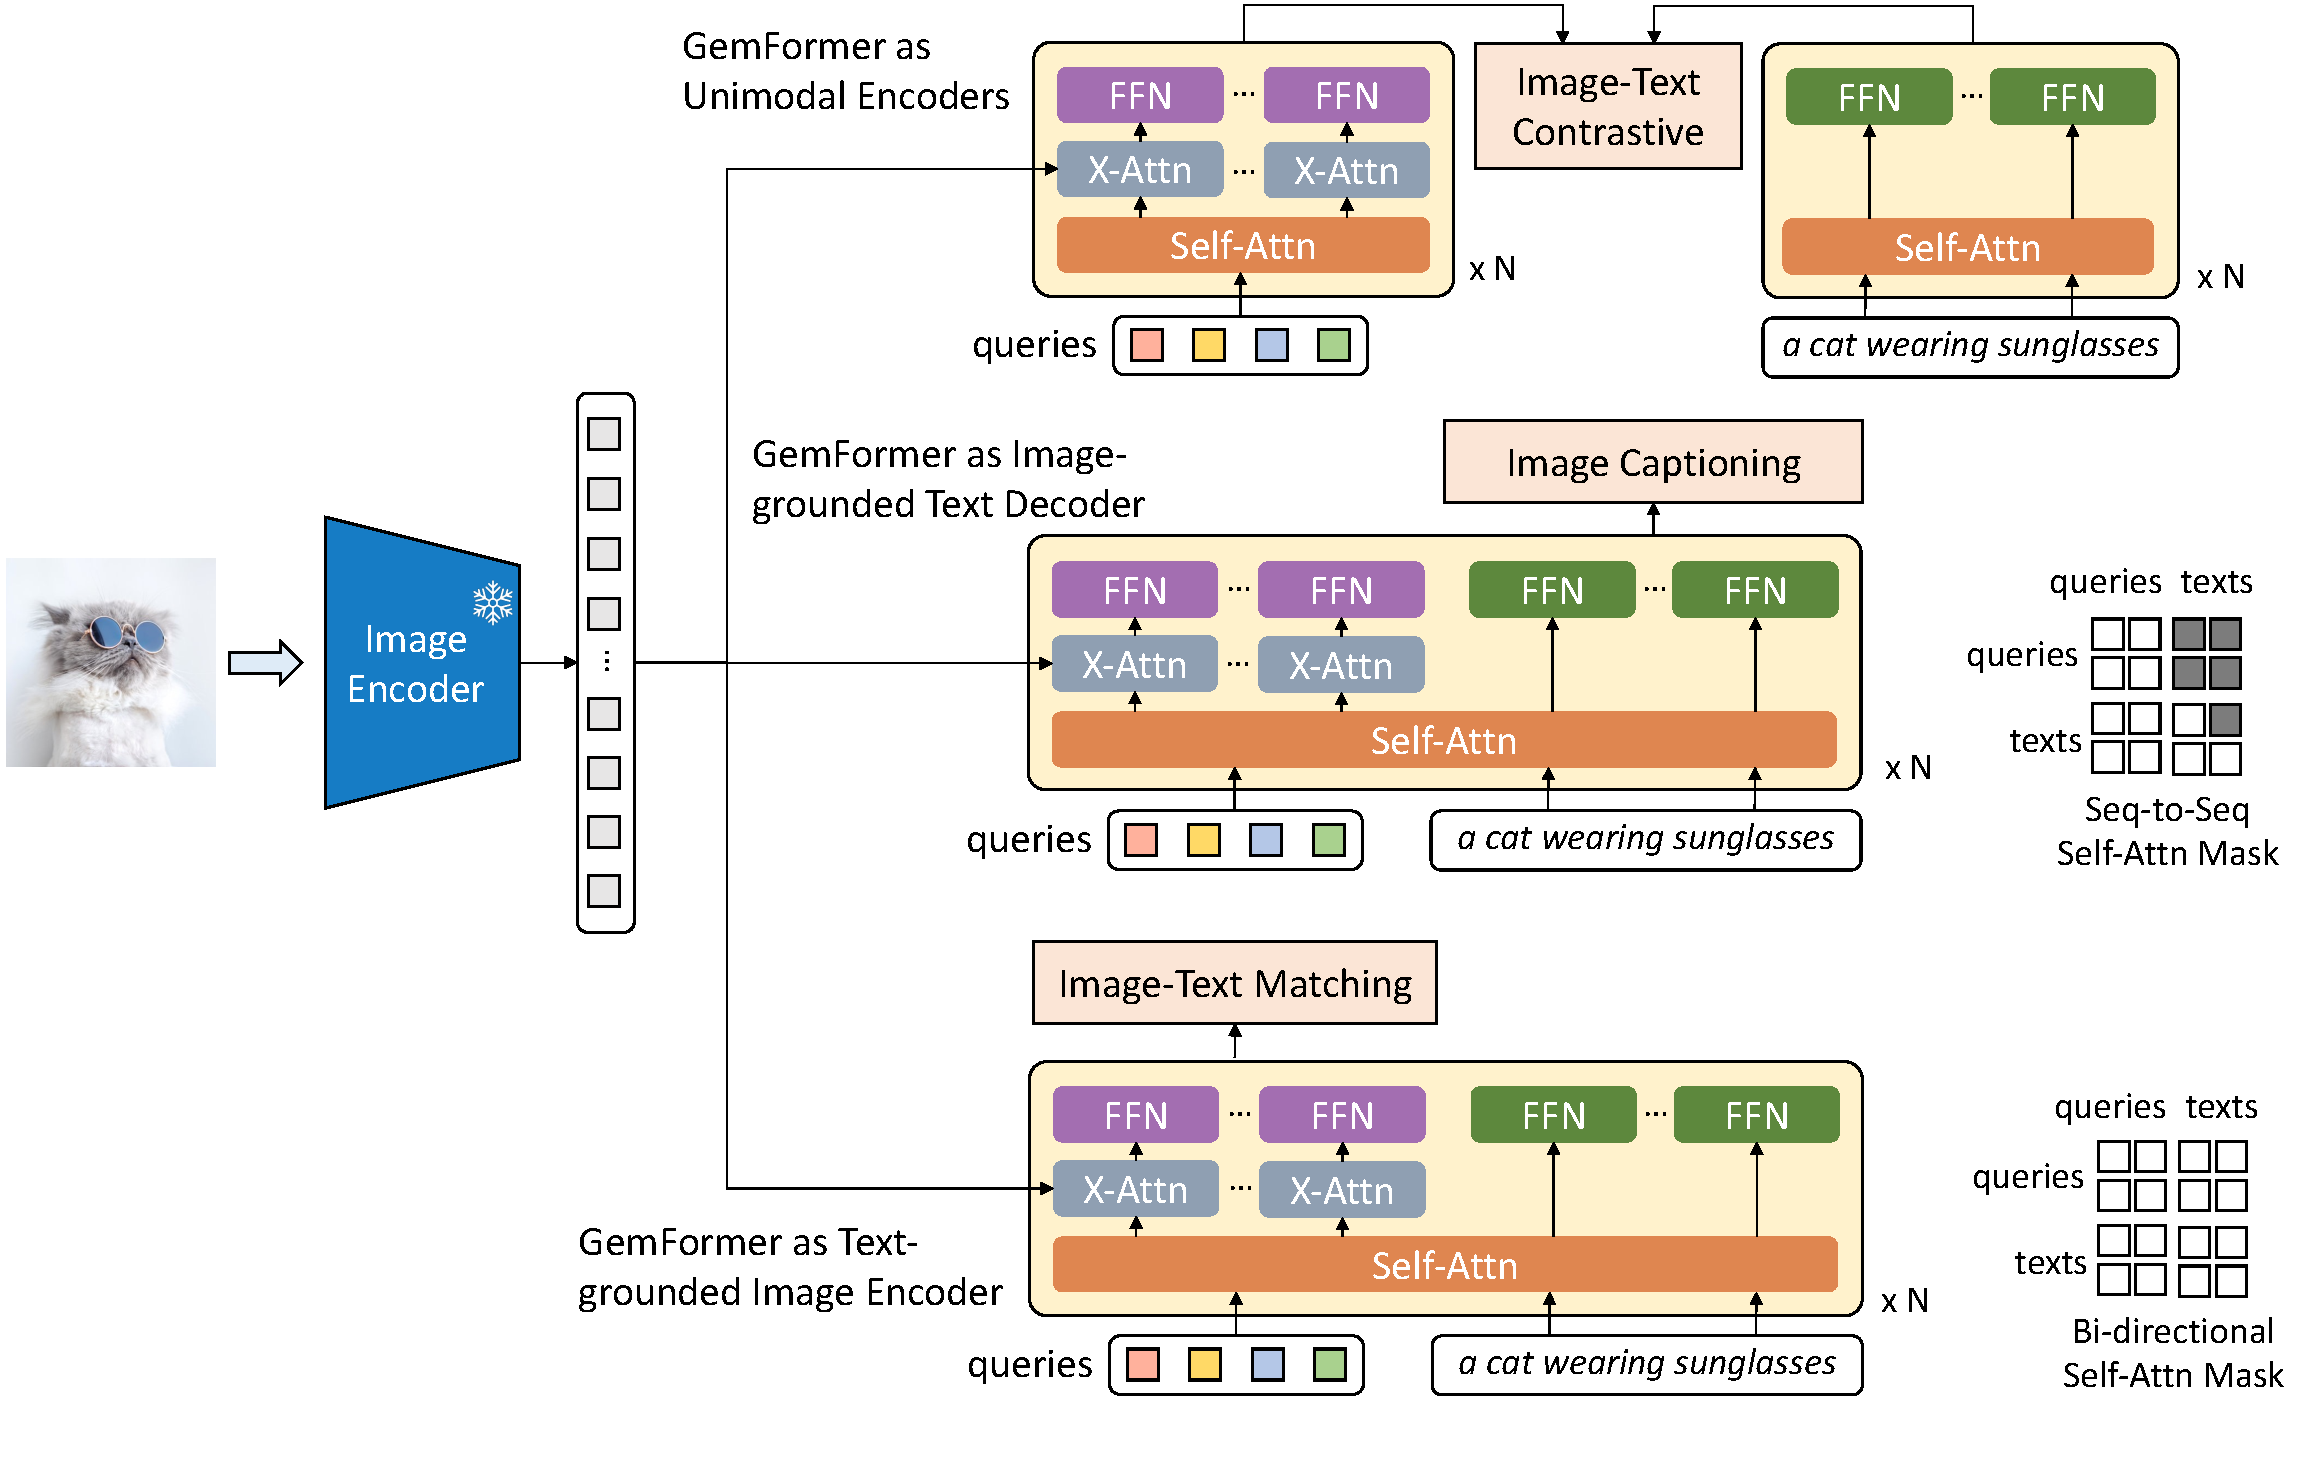
\includegraphics[width=\textwidth]{image/stage1.pdf}
% %   
\includegraphics[width=\textwidth]{BLIPv2/image/fig2.pdf}
% %   
\includegraphics[width=\textwidth]{BLIPv2/image/fig2-v2.pdf}
% % \vspace{-2ex}
% \caption{Pre-training.
% }
% %\vspace{-1ex}
% \label{fig:stage1}
% \end{figure*}

% \begin{figure*}[!t]
% \centering
% %   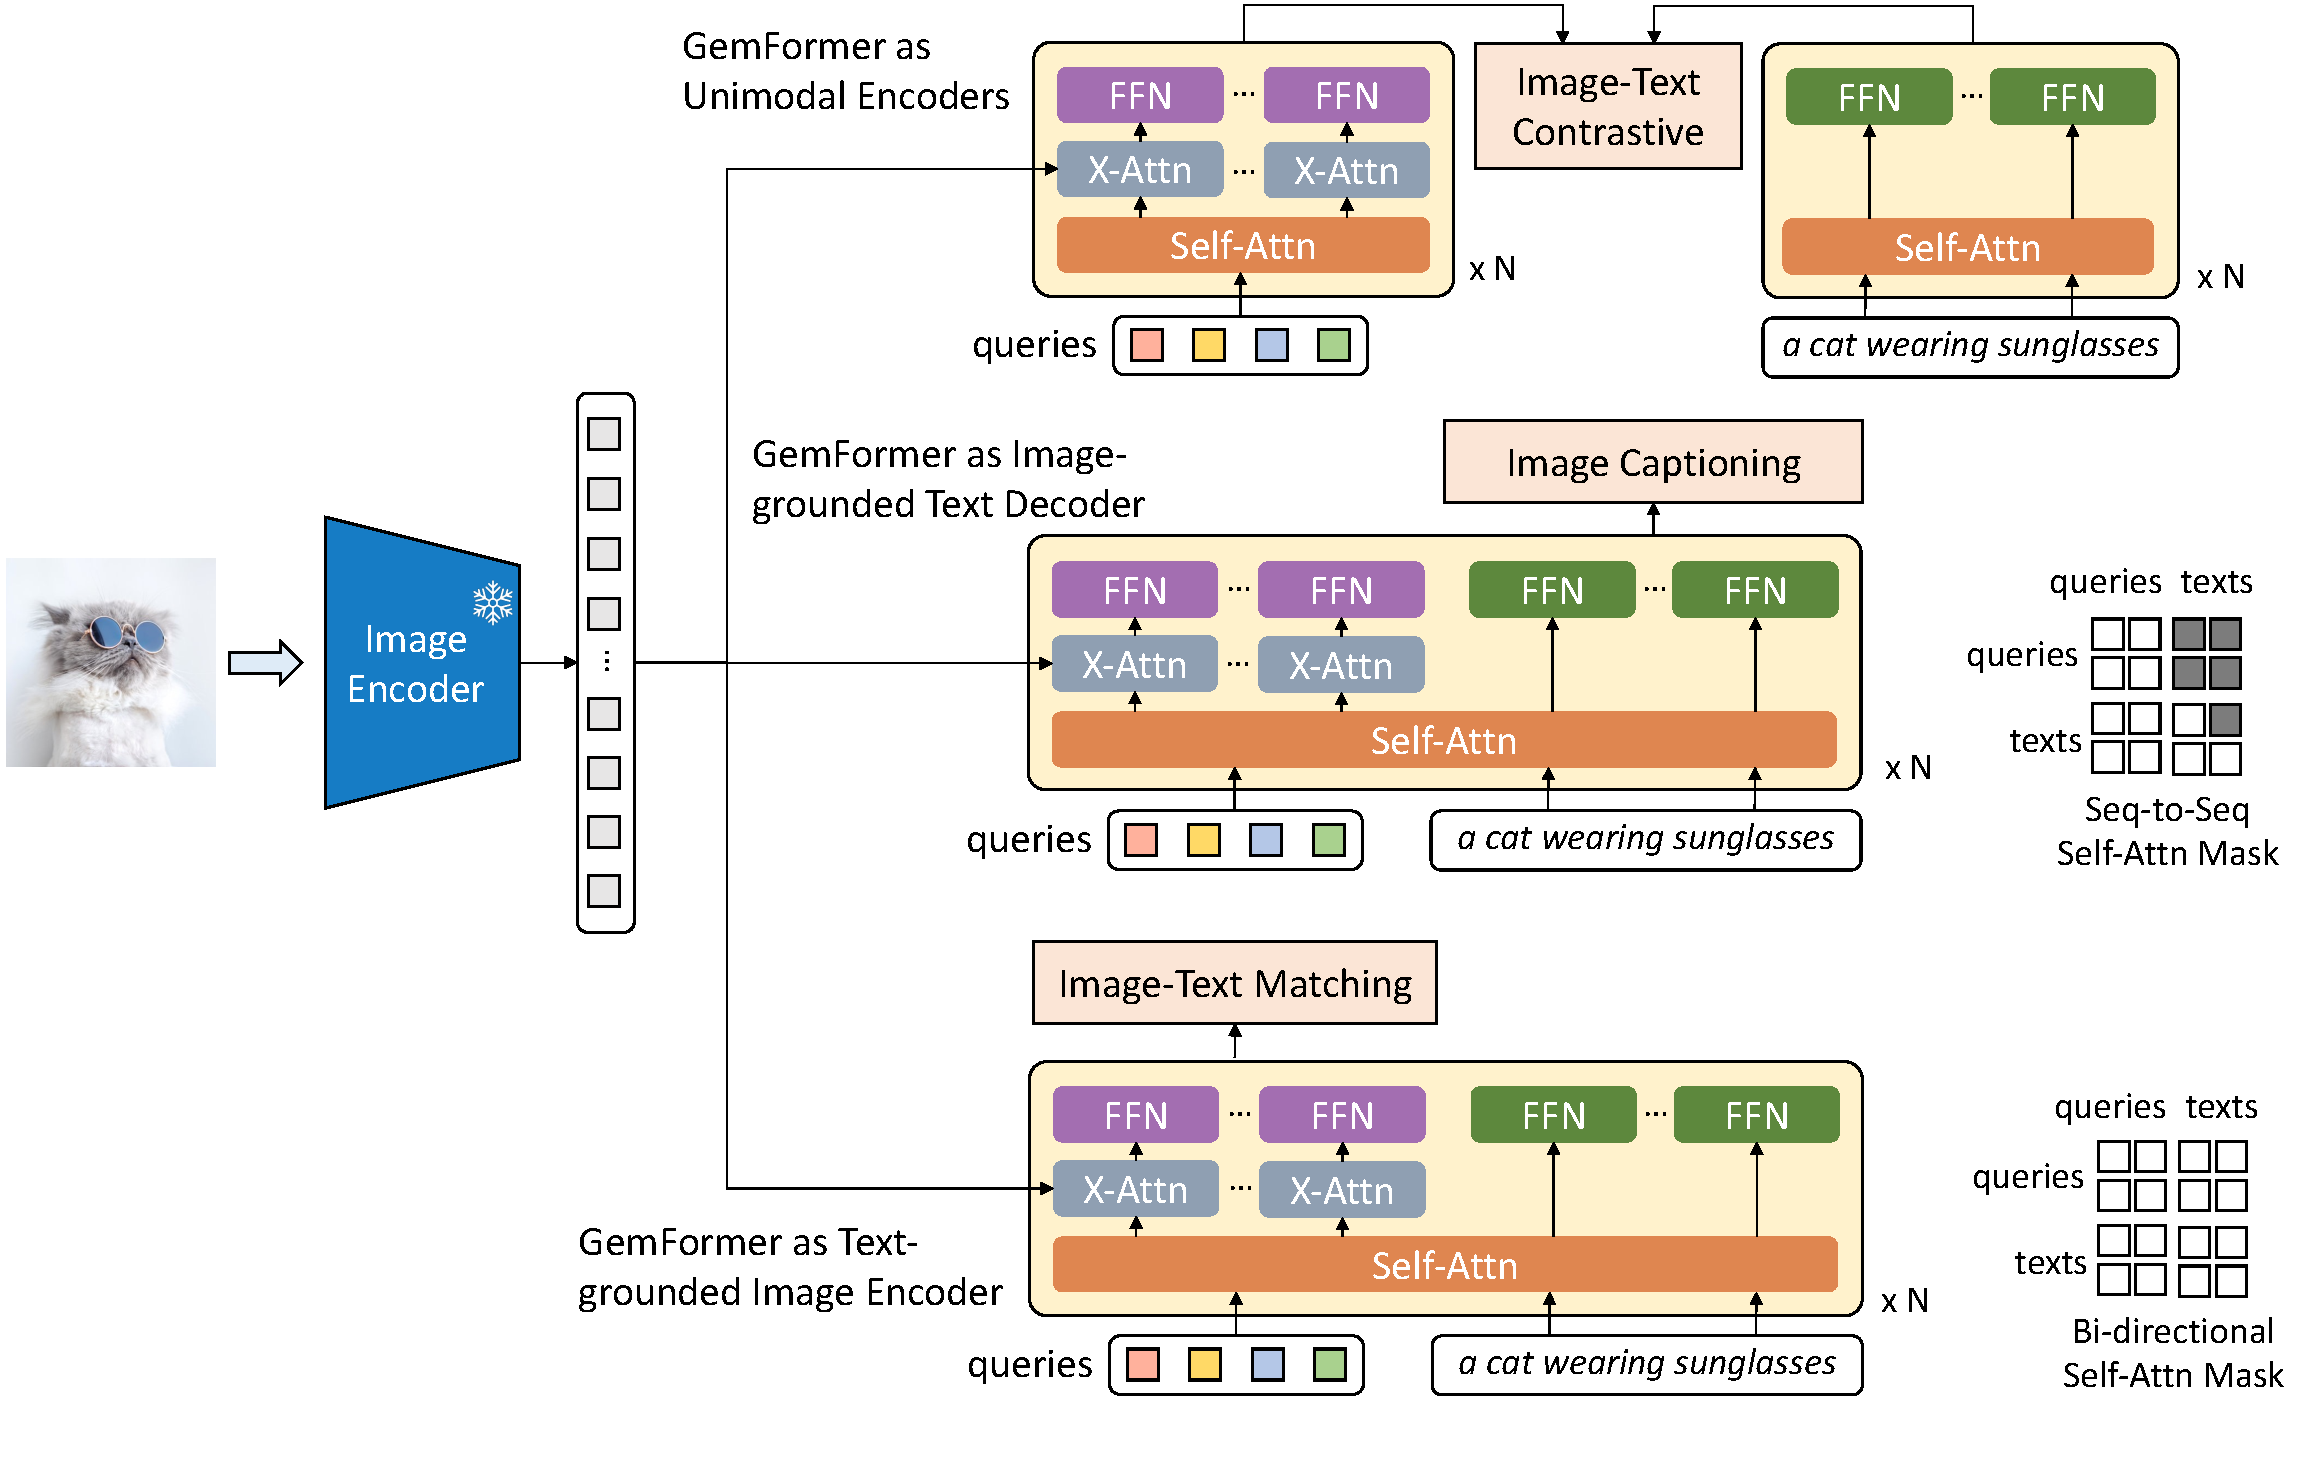
\includegraphics[width=\textwidth]{image/stage1.pdf}
%   
\includegraphics[width=\textwidth]{BLIPv2/image/fig2.pdf}
%   
\includegraphics[width=\textwidth]{BLIPv2/image/fig2-v2.pdf}
% % \vspace{-2ex}
% \caption{Pre-training.
% }
% \end{figure*}

% % \begin{figure*}[!t]
% % \centering
% % %   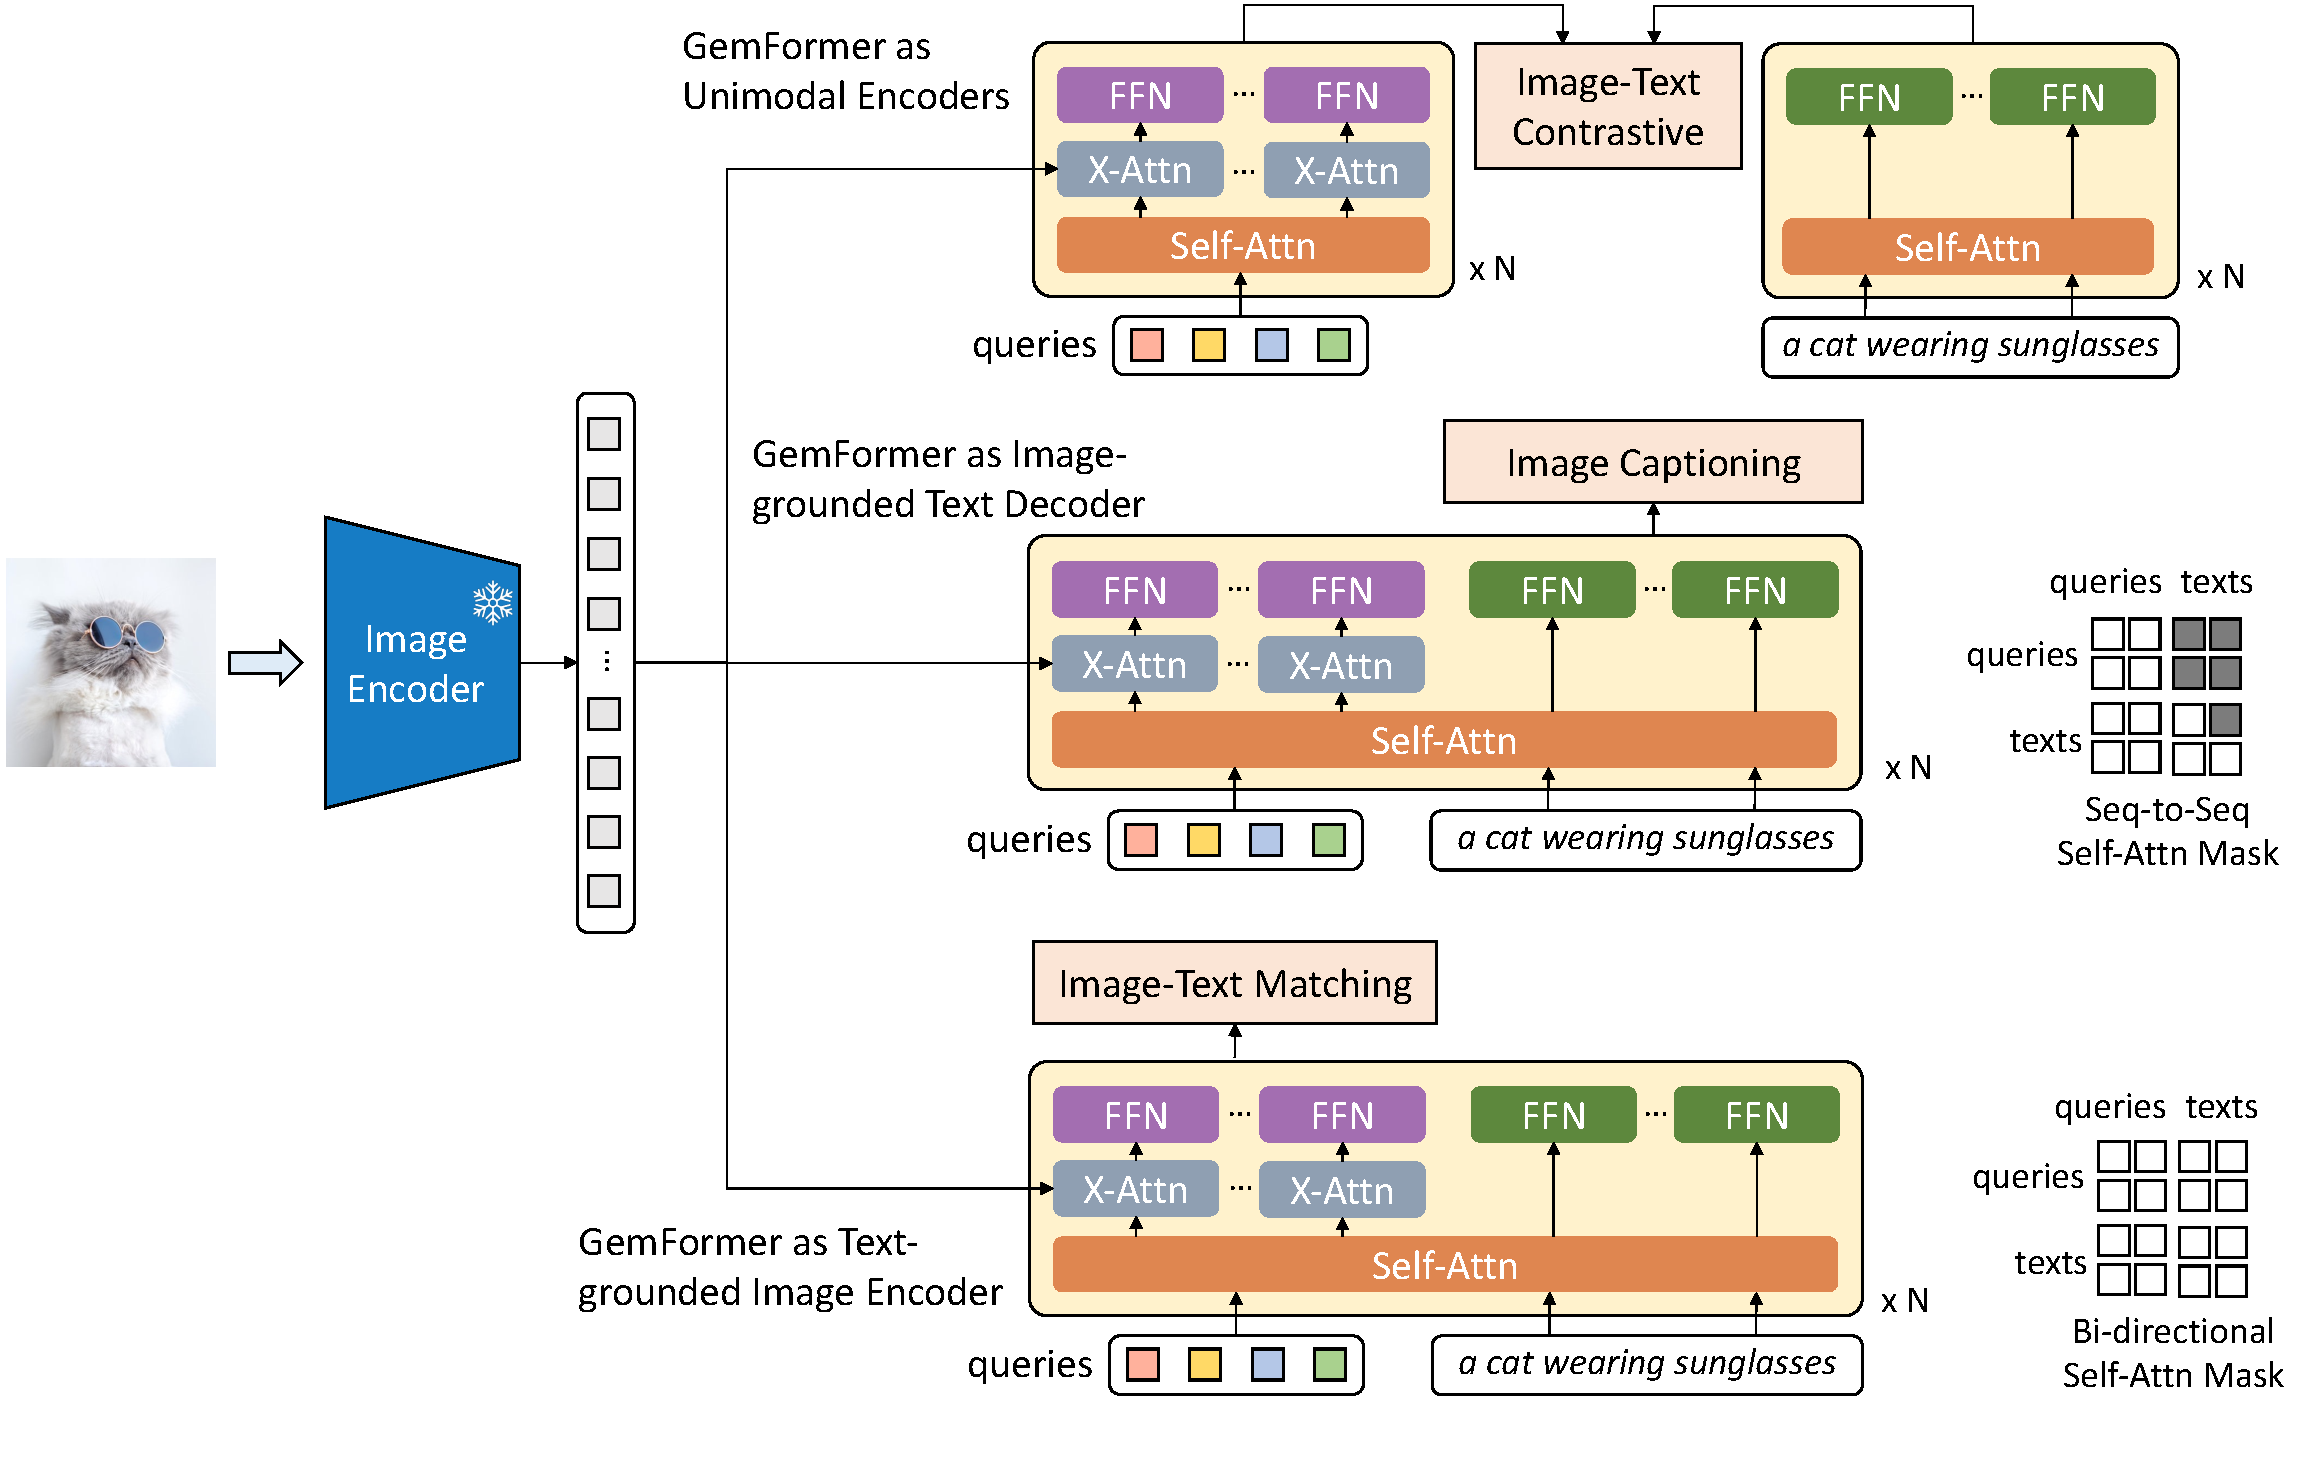
\includegraphics[width=\textwidth]{image/stage1.pdf}
% % %   
\includegraphics[width=\textwidth]{BLIPv2/image/fig2.pdf}
% %   
\includegraphics[width=\textwidth]{BLIPv2/image/fig2-v2.pdf}
% % % \vspace{-2ex}
% % \caption{Pre-training.
% % }
% %\vspace{-1ex}
% % \label{fig:stage1}
% % \end{figure*}

% % \newpage
% \begin{figure*}[!t]
% \centering
% %   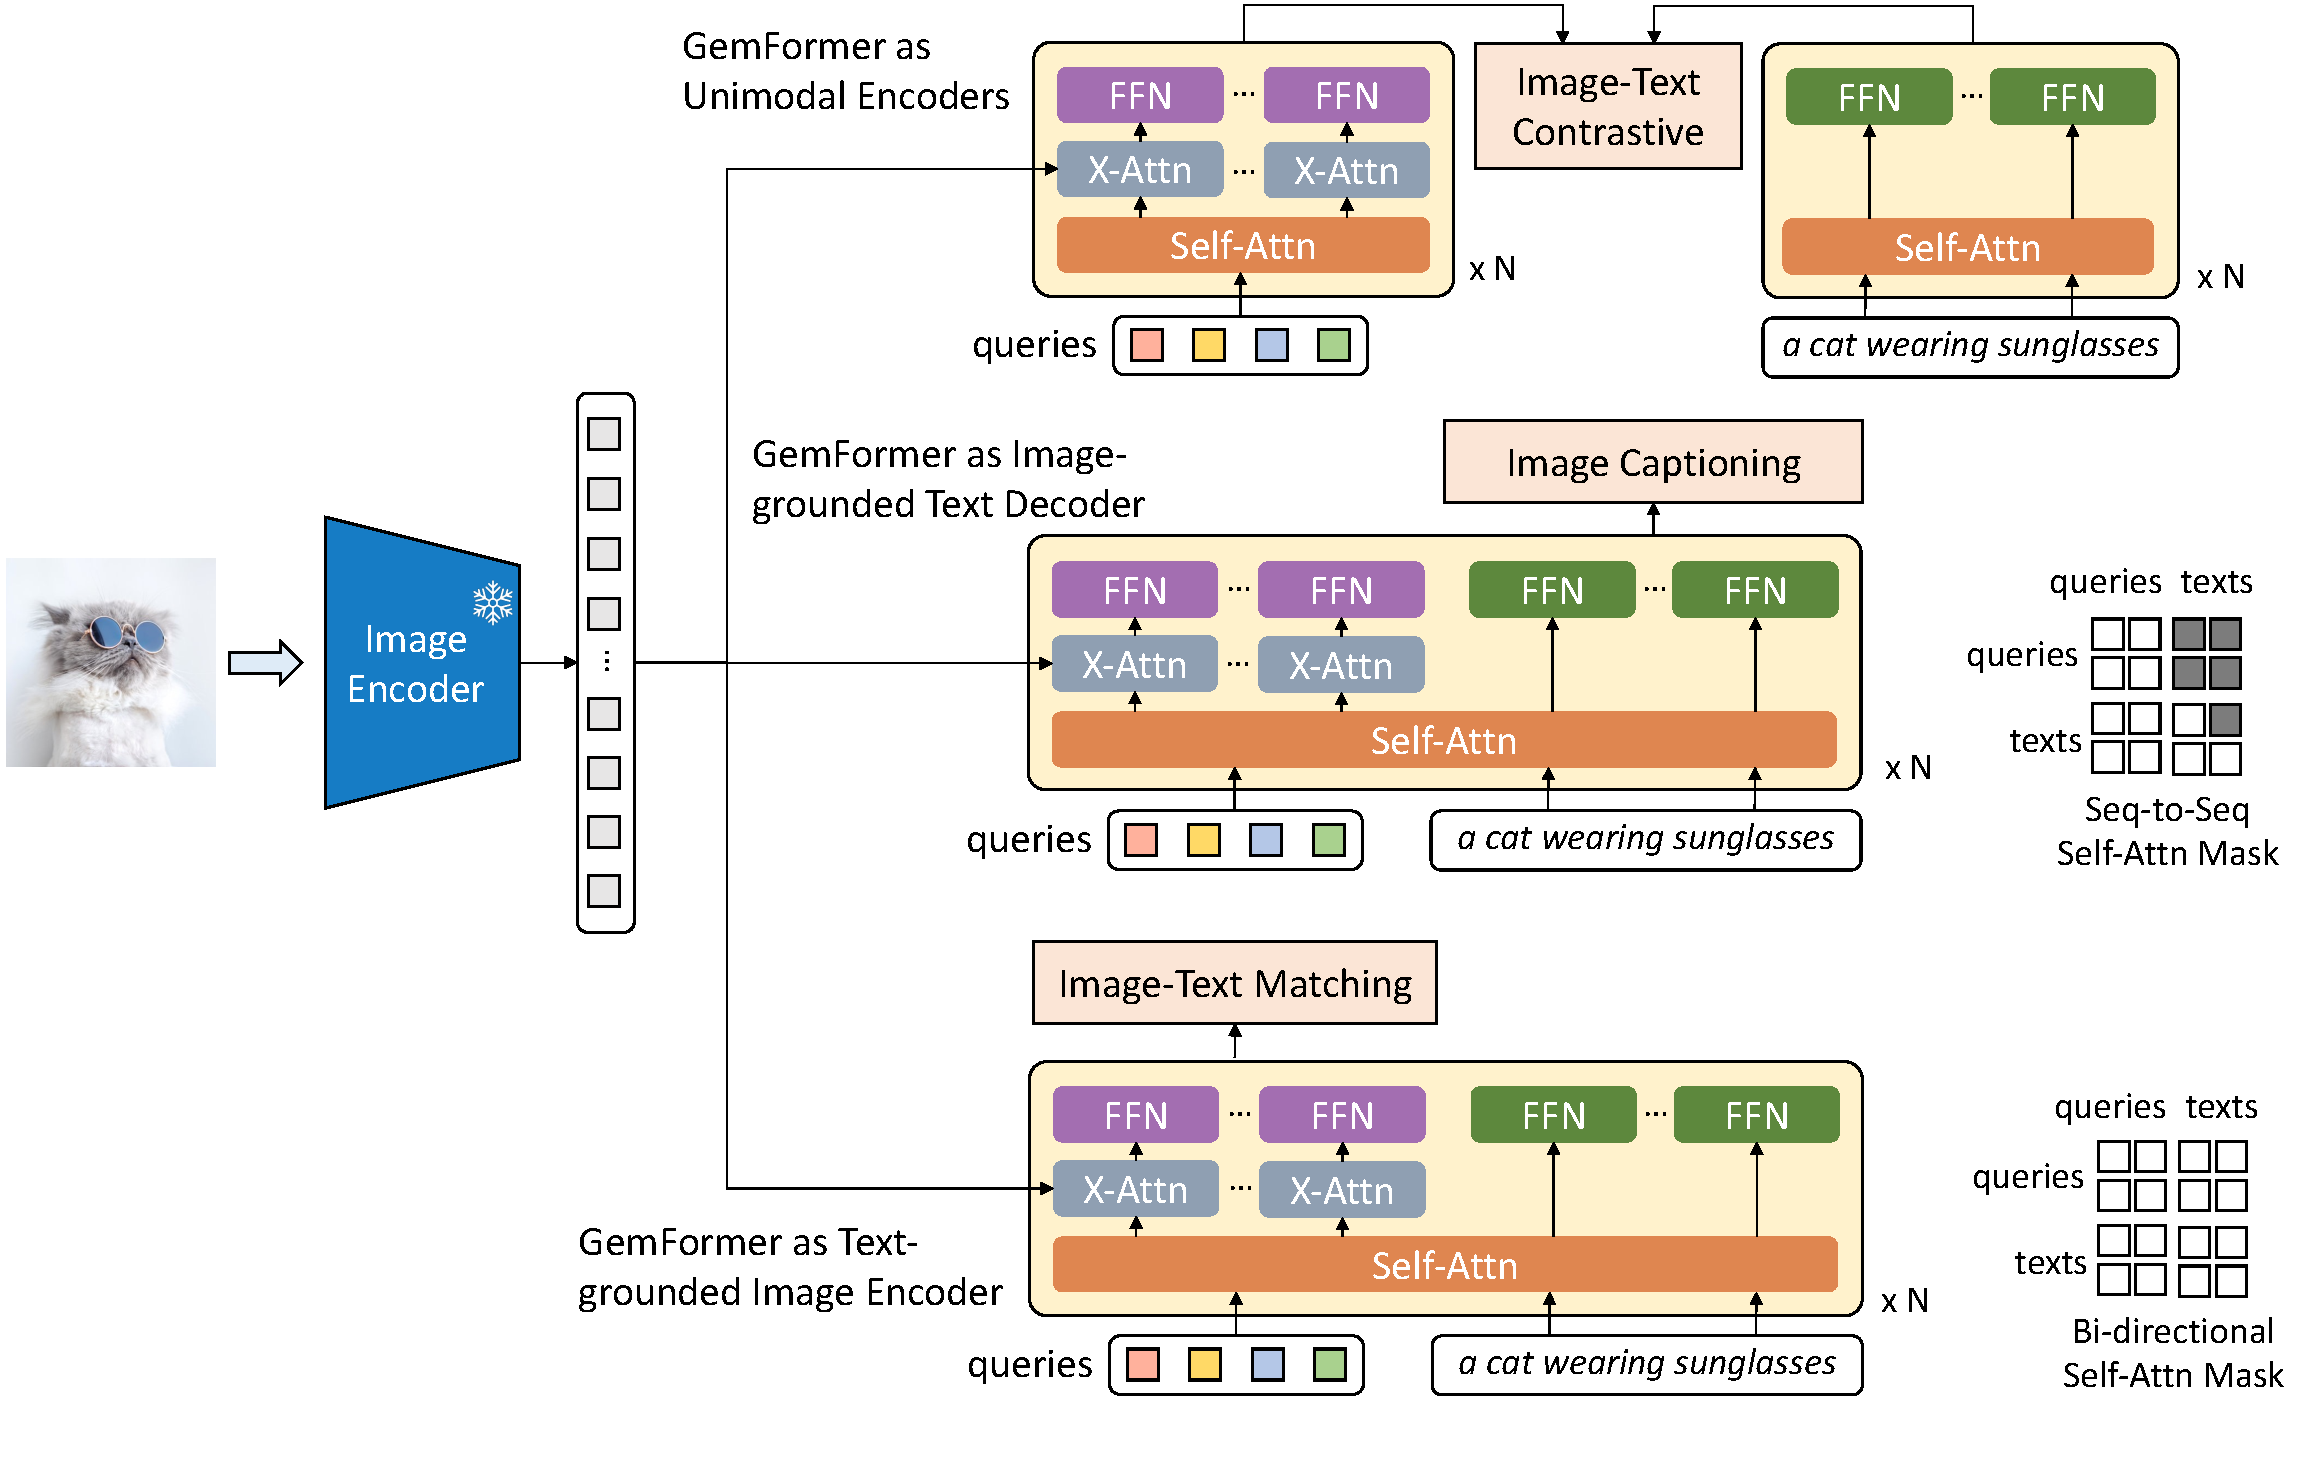
\includegraphics[width=\textwidth]{image/stage1.pdf}
%   
\includegraphics[width=\textwidth]{BLIPv2/image/fig2-v3.pdf}
% % \vspace{-2ex}
% \caption{Pre-training.}
% %\vspace{-1ex}
% \label{fig:stage1}
% \end{figure*}

% \newpage
\begin{figure*}[!t]
% \centering
%   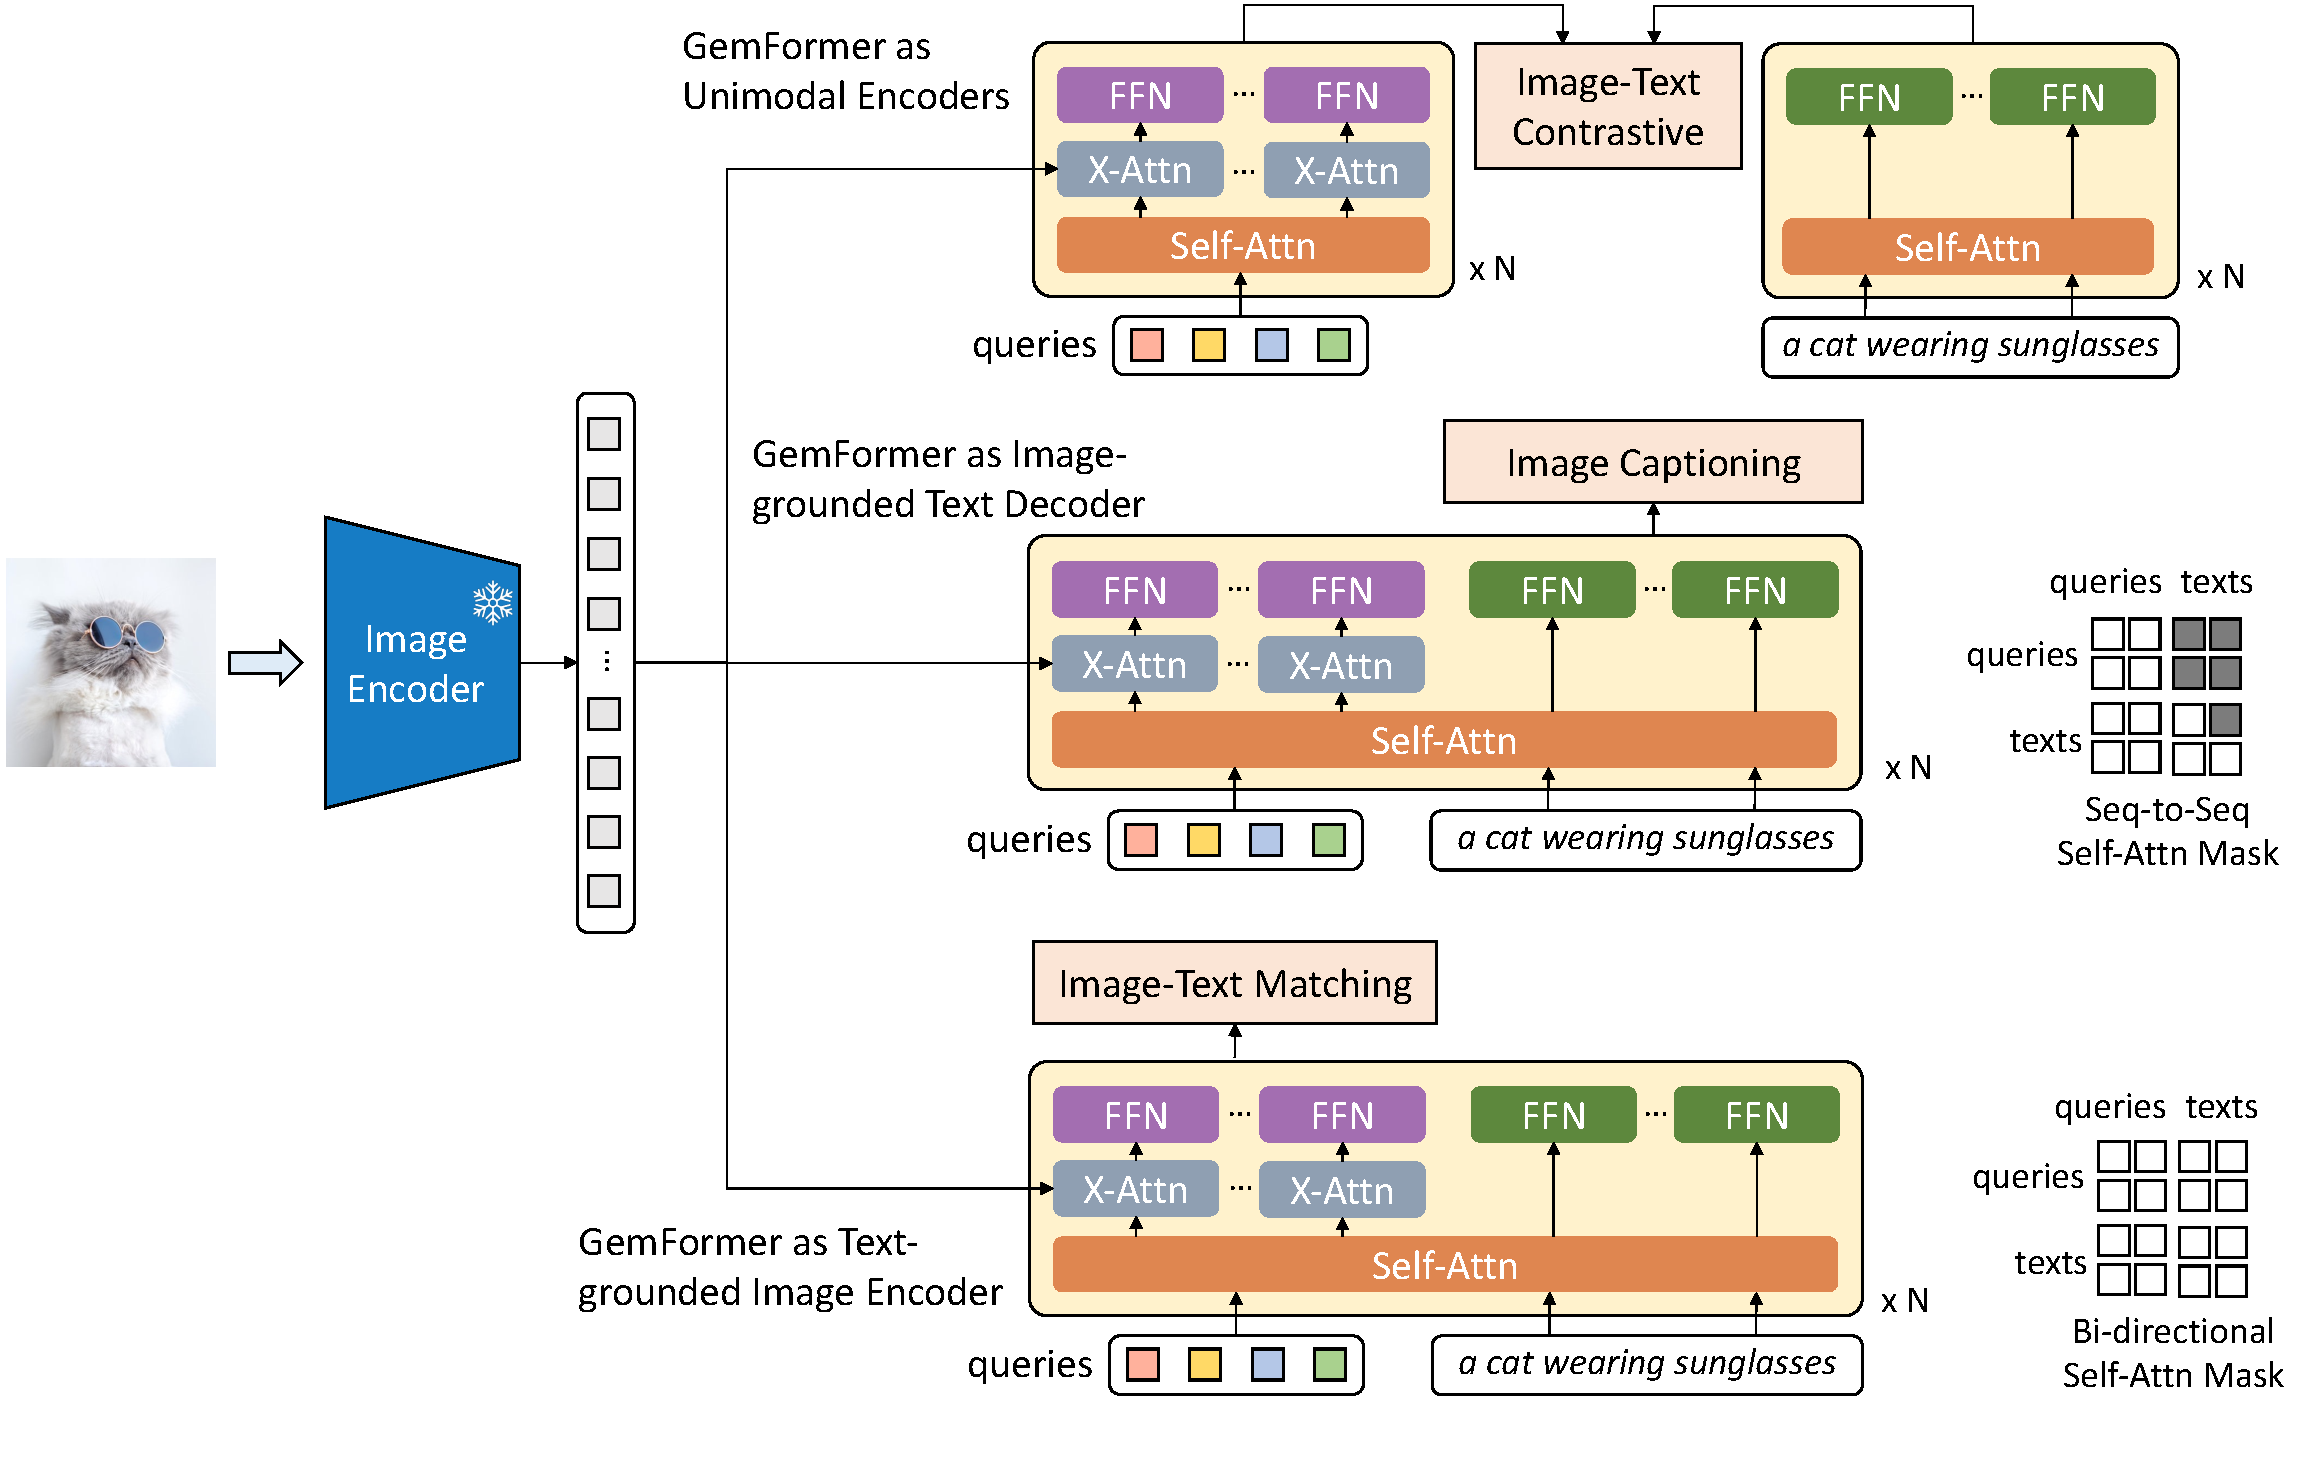
\includegraphics[width=\textwidth]{image/stage1.pdf}
  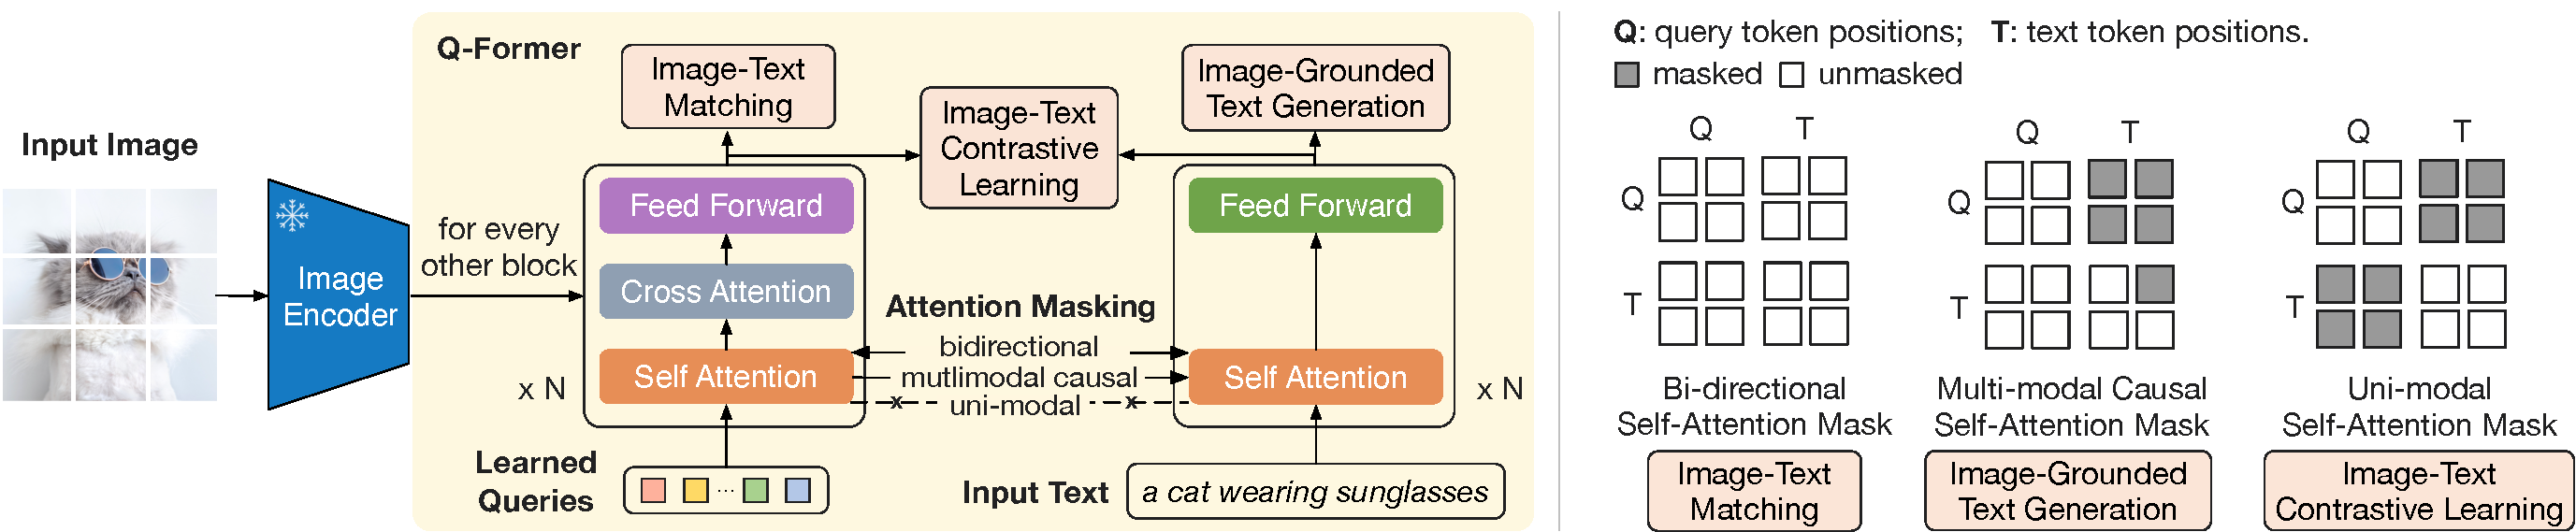
\includegraphics[width=\textwidth]{image/fig2-v5.pdf}
\vspace{-3.5ex}
\caption{(\textbf{Left}) Model architecture of \name~and BLIP-2's first-stage vision-language representation learning objectives. We jointly optimize three objectives which enforce the queries (a set of learnable embeddings) to extract visual representation most relevant to the text. (\textbf{Right}) The self-attention masking strategy for each objective to control query-text interaction.}
\vspace{-1.5ex}
\label{fig:stage1}
\end{figure*}

We propose BLIP-2, a new vision-language pre-training method that bootstraps from frozen pre-trained unimodal models.
In order to bridge the modality gap,
we propose a Querying Transformer (\name) pre-trained in two stages:
(1) vision-language representation learning stage with a frozen image encoder and (2) vision-to-language generative learning stage with a frozen LLM.
% The core of our method is a Querying Transformer (\name).
% \name~can connect to a frozen pre-trained image encoder at one end to perform vision-language representation learning.
% It can also connect to a frozen pre-trained LLM at the other end to perform vision-to-language generative learning.
This section first introduces the model architecture of \name,
and then delineates the two-stage pre-training procedures.

\vspace{-0.5ex}
\subsection{Model Architecture}
\vspace{-0.5ex}
We propose \name~as the trainable module to bridge the gap between a frozen image encoder and a frozen LLM.
It extracts a fixed number of output features from the image encoder,
independent of input image resolution.
As shown in Figure~\ref{fig:stage1},
\name~consists of two transformer submodules that share the same self-attention layers: (1) an image transformer that interacts with the frozen image encoder for visual feature extraction, (2) a text transformer that can function as both a text encoder and a text decoder.
We create a set number of learnable query embeddings as input to the image transformer.
%
The queries interact with each other through self-attention layers, and interact with frozen image features through cross-attention layers (inserted every other transformer block).
The queries can additionally interact with the text through the same self-attention layers.
Depending on the pre-training task,
we apply different self-attention masks to control query-text interaction.
% This interaction can be unidirectional (from query to text) or bidirectional.
We initialize \name~with the pre-trained weights of BERT$_\text{base}$~\cite{bert}, whereas the cross-attention layers are randomly initialized. 
In total, \name~contains 188M parameters.
Note that the queries are considered as model parameters.

In our experiments,
we use 32 queries where each query has a dimension of 768 (same as the hidden dimension of the \name).
We use $Z$ to denote the output query representation.
The size of $Z$ ($32\times768$) is much smaller than the size of frozen image features (\eg~$257\times1024$ for ViT-L/14).
This bottleneck architecture works together with our pre-training objectives into forcing the queries to extract visual information that is most relevant to the text.


% An illustration of \name~is shown in Figure~\ref{fig:stage1}.
% It can take three types of inputs:
% (1) image features $I$ from a frozen image encoder,
% (2) text tokens $T$,
% (3) a pair of $I$ and $T$.
% When text is the only input, \name~is the same as a standard language transformer~\cite{bert}.
% In order to process frozen image features,
% we create a fixed number of \textit{learnable query embeddings} and pass them as input to \name.
% The queries interact with the image features through additional cross-attention layers (inserted every $N=2$ transformer blocks) and output image representation $Z$.
% The size of $Z$ is much smaller than the size of $I$.
% For example, ViT-L/14~\cite{clip} outputs $I$ of size $257\times1024$,
% whereas $Z$ only has a size of $32\times768$.
% % the same size as the hidden dimension of the transformer.

% The queries interact with each other and the text through self-attention layers.
% We $\textit{decouple}$ the image-text interaction into image-query interaction and query-text interaction.
% This mechanism works together with our pre-training objectives into forcing the queries to extract visual information that is most relevant to the text.

% We initialize \name~with the pre-trained weights of BERT$_\text{base}$~\cite{bert},
% whereas the cross-attention layers are randomly initialized.
% We decouple the feed-forward (FFW) layers for query and text to create two sets of FFWs with different parameters.
% In total, \name~contains 188M parameters.

% \subsection{
\includegraphics[height=0.3cm,trim={0 3cm 0 0}]{image/snowflake2} Image Encoder $\rightarrow$ 
\includegraphics[trim={0 4cm 4cm 0},clip,height=0.4cm]{image/fire} \name}
\vspace{-0.5ex}
\subsection{Bootstrap Vision-Language Representation Learning from a Frozen Image Encoder}
\vspace{-0.5ex}
% An illustration of the first-stage pre-training is shown in Figure~\ref{fig:stage1}.
In the representation learning stage, 
we connect \name~to a frozen image encoder and perform pre-training using image-text pairs.
% We design our pre-training objectives such that the \name learns the following capabilities:
% (1) Given an image, extract visual representation that has the largest mutual information with the corresponding text.
% (2) Given an image, generate the corresponding text.
% (2) Given an image-text pair, extract language-informed visual representation.
% The resulting \name~thereby can function as an information bottleneck between the image encoder and the LLM,
% which removes irrelevant information from input to the LLM and mitigates overfitting.
% (1) the queries should extract visual information that is most relevant to the text,
% (2) the queries should learn the interaction between images and texts and be able to extract visual information while conditioned on the text.
We aim to train the \name~such that the queries can learn to extract visual representation that is most informative of the text.
Inspired by BLIP~\cite{blip}, we jointly optimize three pre-training objectives that share the same input format and model parameters.
Each objective employs a different attention masking strategy between queries and text to control their interaction (see Figure~\ref{fig:stage1}).

% To this end, we re-invent the following pre-training objectives from BLIP~\cite{blip}.
% An illustration is shown in Figure~\ref{fig:stage1}.
% Next we explain the details.

\noindent\textbf{Image-Text Contrastive Learning} (ITC) learns to align image representation and text representation such that their mutual information is maximized.
It achieves so by contrasting the image-text similarity of a positive pair against those of negative pairs.
% Existing dual-encoder methods apply the ITC loss to align the unimodal representation from the image encoder and text encoder, respectively~\cite{clip,align,ALBEF,blip}.
% Different from these methods,
We align the output query representation $Z$ from the image transformer with the text representation $t$ from the text transformer,
where $t$ is the output embedding of the \texttt{[CLS]} token.
Since $Z$ contains multiple output embeddings (one from each query),
we first compute the pairwise similarity between each query output and $t$, and then select the highest one as the image-text similarity.
To avoid information leak, we employ a unimodal self-attention mask,
where the queries and text are not allowed to see each other.
Due to the use of a frozen image encoder, we can fit more samples per GPU compared to end-to-end methods.
Therefore, we use in-batch negatives instead of the momentum queue in BLIP.


\noindent\textbf{Image-grounded Text Generation} (ITG) loss trains the \name~to generate texts, given input images as the condition.
Since the architecture of \name~does not allow direct interactions between the frozen image encoder and the text tokens,
the information required for generating the text must be first extracted by the queries,
and then passed to the text tokens via self-attention layers.
Therefore, the queries are forced to extract visual features that capture all the information about the text. 
We employ a multimodal causal self-attention mask to control query-text interaction, similar to the one used in UniLM~\cite{UniLM}.
The queries can attend to each other but not the text tokens.
Each text token can attend to all queries and its previous text tokens.
We also replace the \texttt{[CLS]} token with a new \texttt{[DEC]} token as the first text token to signal the decoding task.


\noindent\textbf{Image-Text Matching} (ITM)
aims to learn fine-grained alignment between image and text representation.
It is a binary classification task where the model is asked to predict whether an image-text pair is positive
(matched) or negative (unmatched).
We use a bi-directional self-attention mask where all queries and texts can attend to each other.
The output query embeddings $Z$ thus capture multimodal information.
We feed each output query embedding into a two-class linear classifier to obtain a logit,
and average the logits across all queries as the output matching score.
We adopt the hard negative mining strategy from~\citet{ALBEF,blip} to create informative negative pairs.

% \subsection{
\includegraphics[height=0.3cm,trim={0 3cm 0 0}]{image/snowflake2} Image Encoder $\rightarrow$ 
\includegraphics[trim={0 4cm 4cm 0},clip,height=0.4cm]{image/fire} \name $\rightarrow$ 
\includegraphics[height=0.3cm,trim={0 3cm 0 0}]{image/snowflake2}LLM}

% \begin{figure*}[!t]
% \centering
%   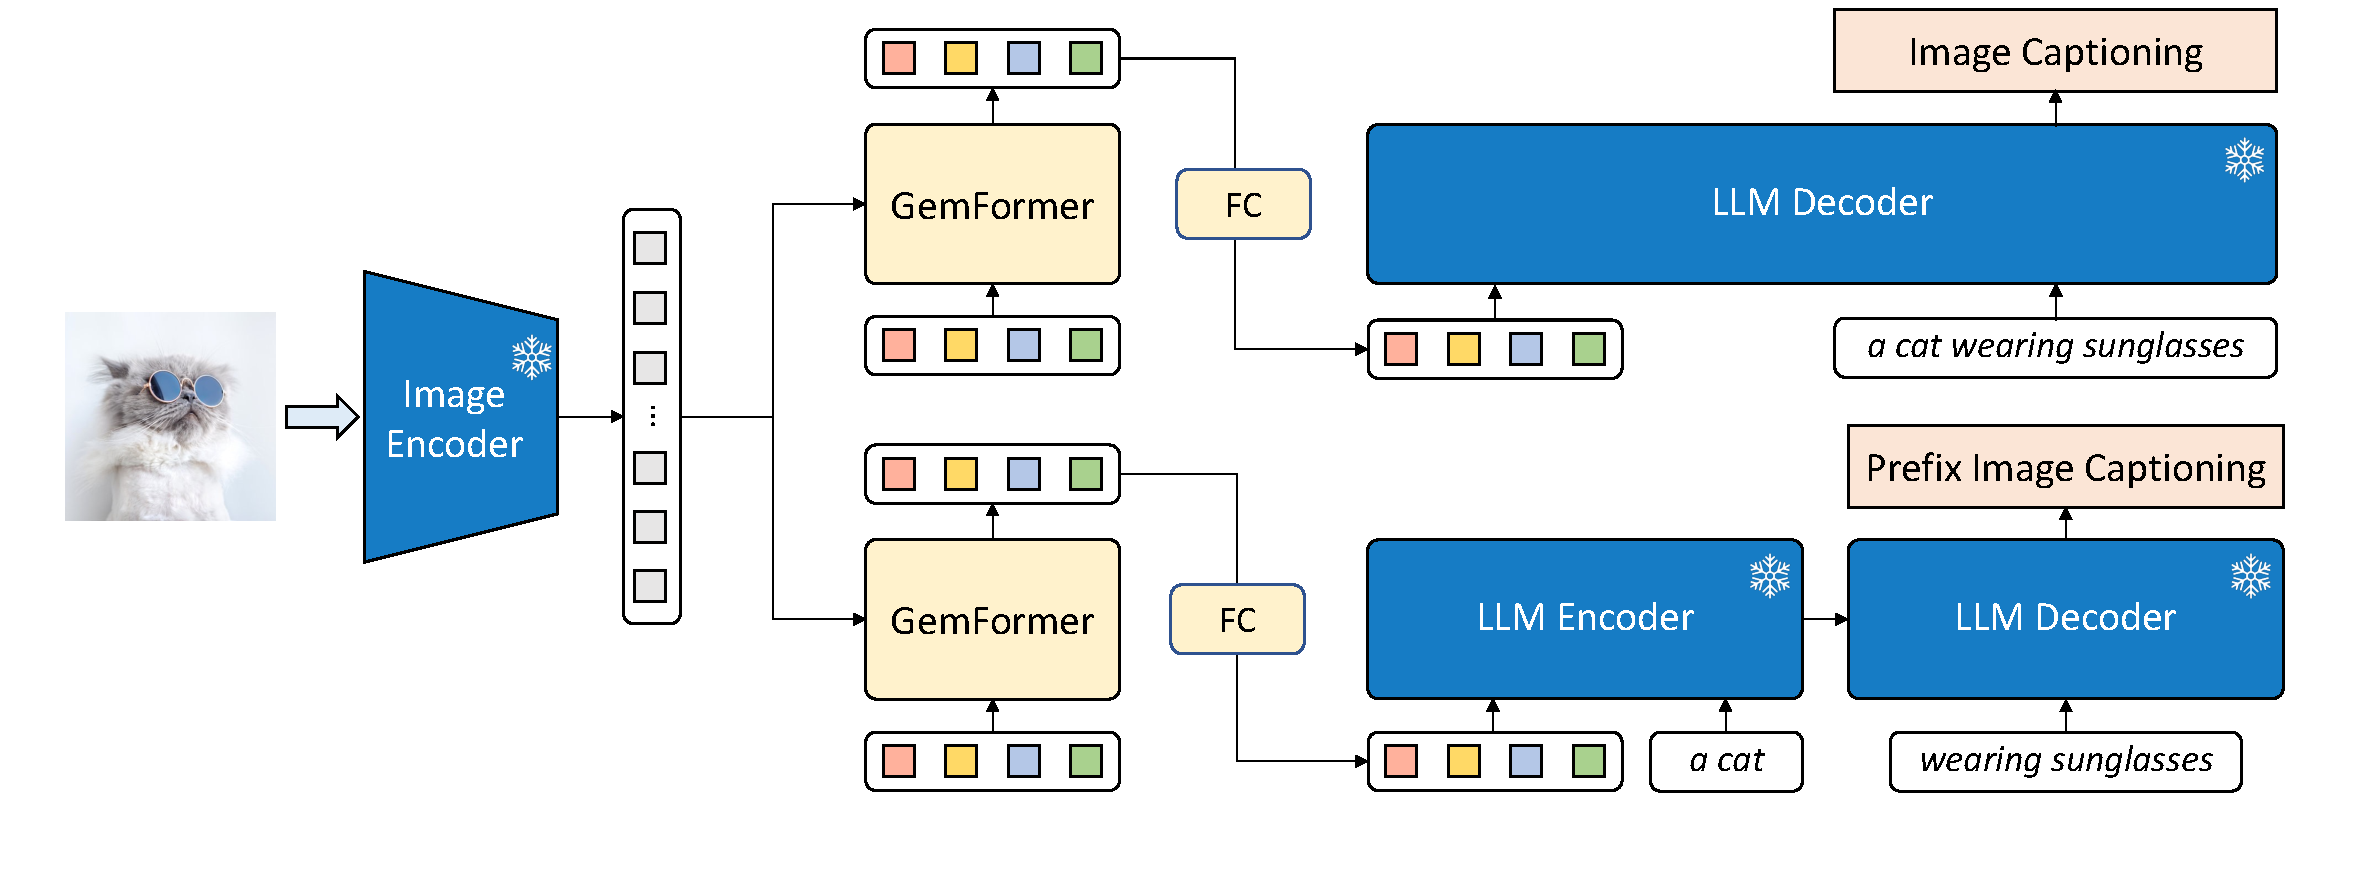
\includegraphics[width=\textwidth]{image/stage2.pdf}
% \vspace{-2ex}
% \caption{Pre-training.
% }
% %\vspace{-1ex}
% \label{fig:stage2}
% \end{figure*}

% \begin{figure*}[!t]
% \centering
%   
\includegraphics[width=\textwidth]{BLIPv2/image/fig3.pdf}
% \vspace{-2ex}
% \caption{Pre-training.}
% %\vspace{-1ex}
% \label{fig:stage2}
% \end{figure*}


\begin{figure*}[!t]
\centering
%   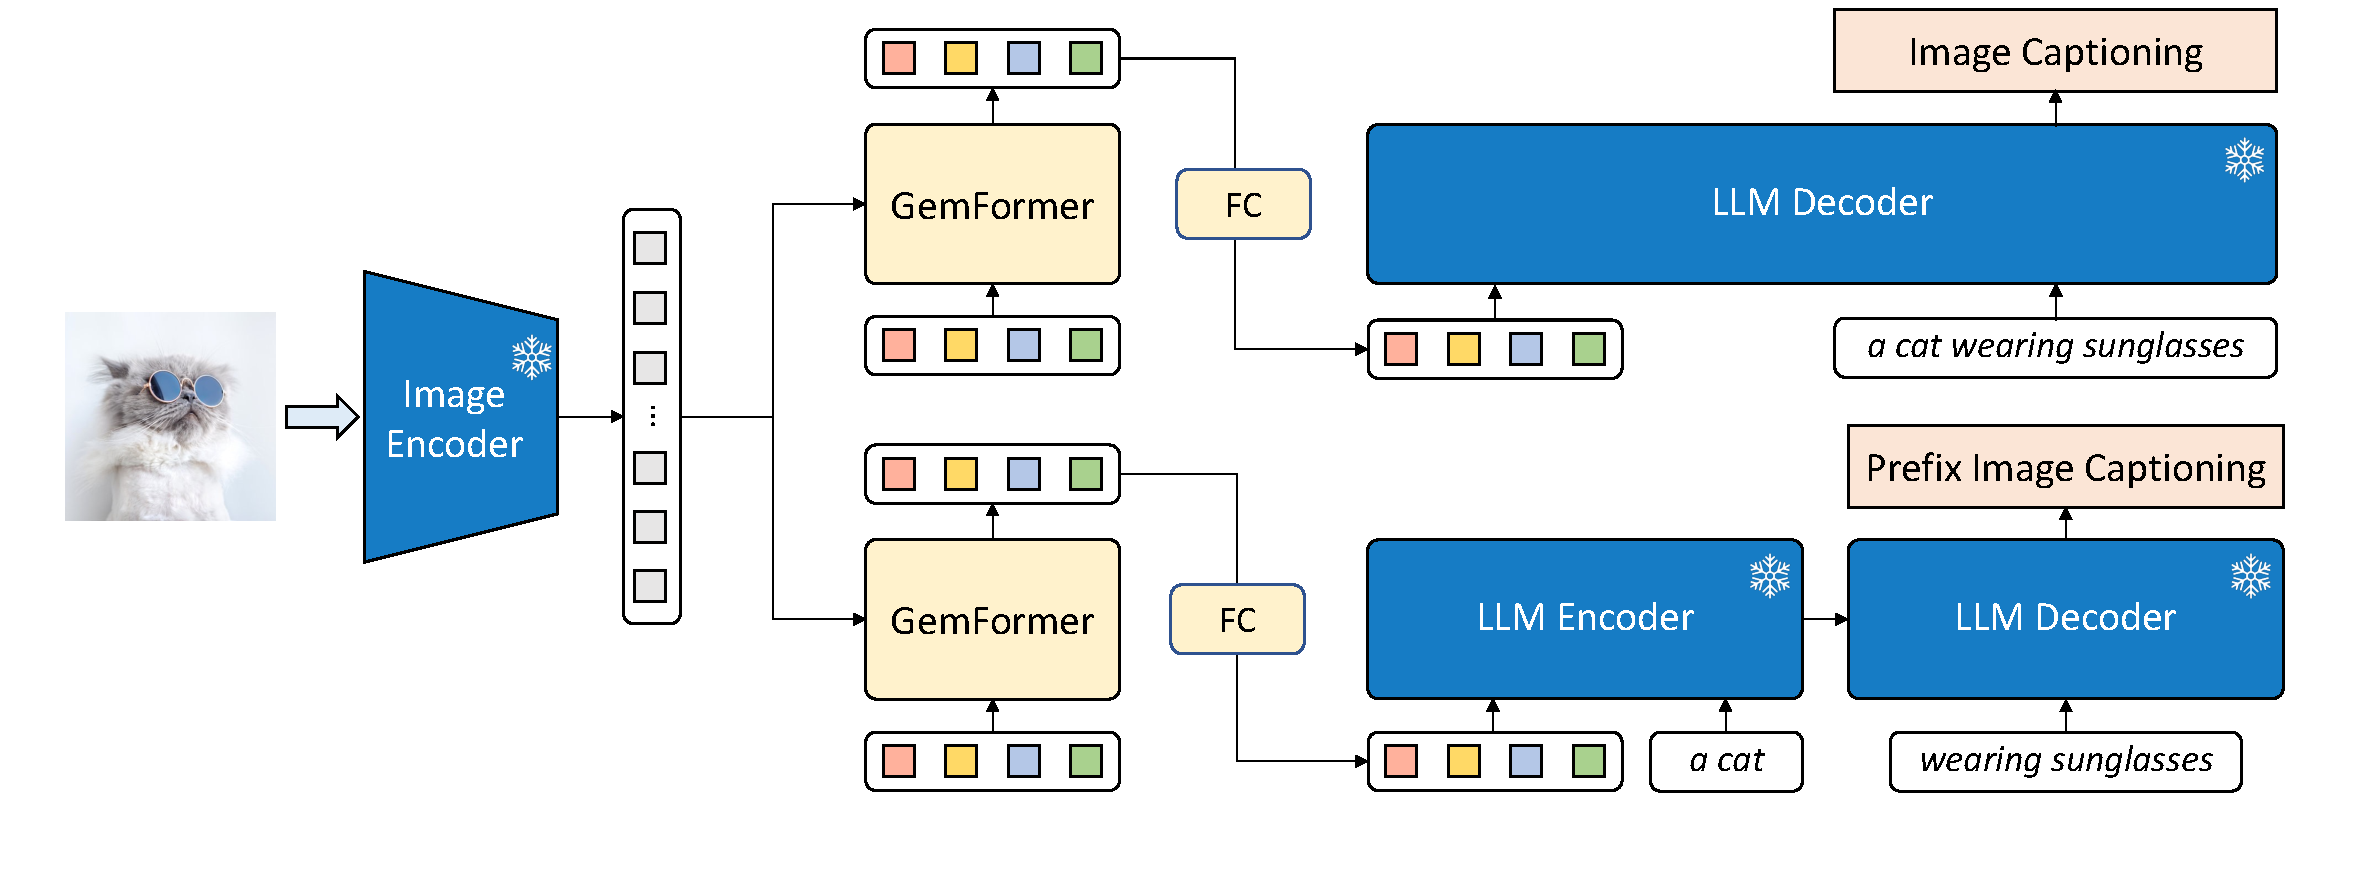
\includegraphics[width=\textwidth]{image/stage2.pdf}
  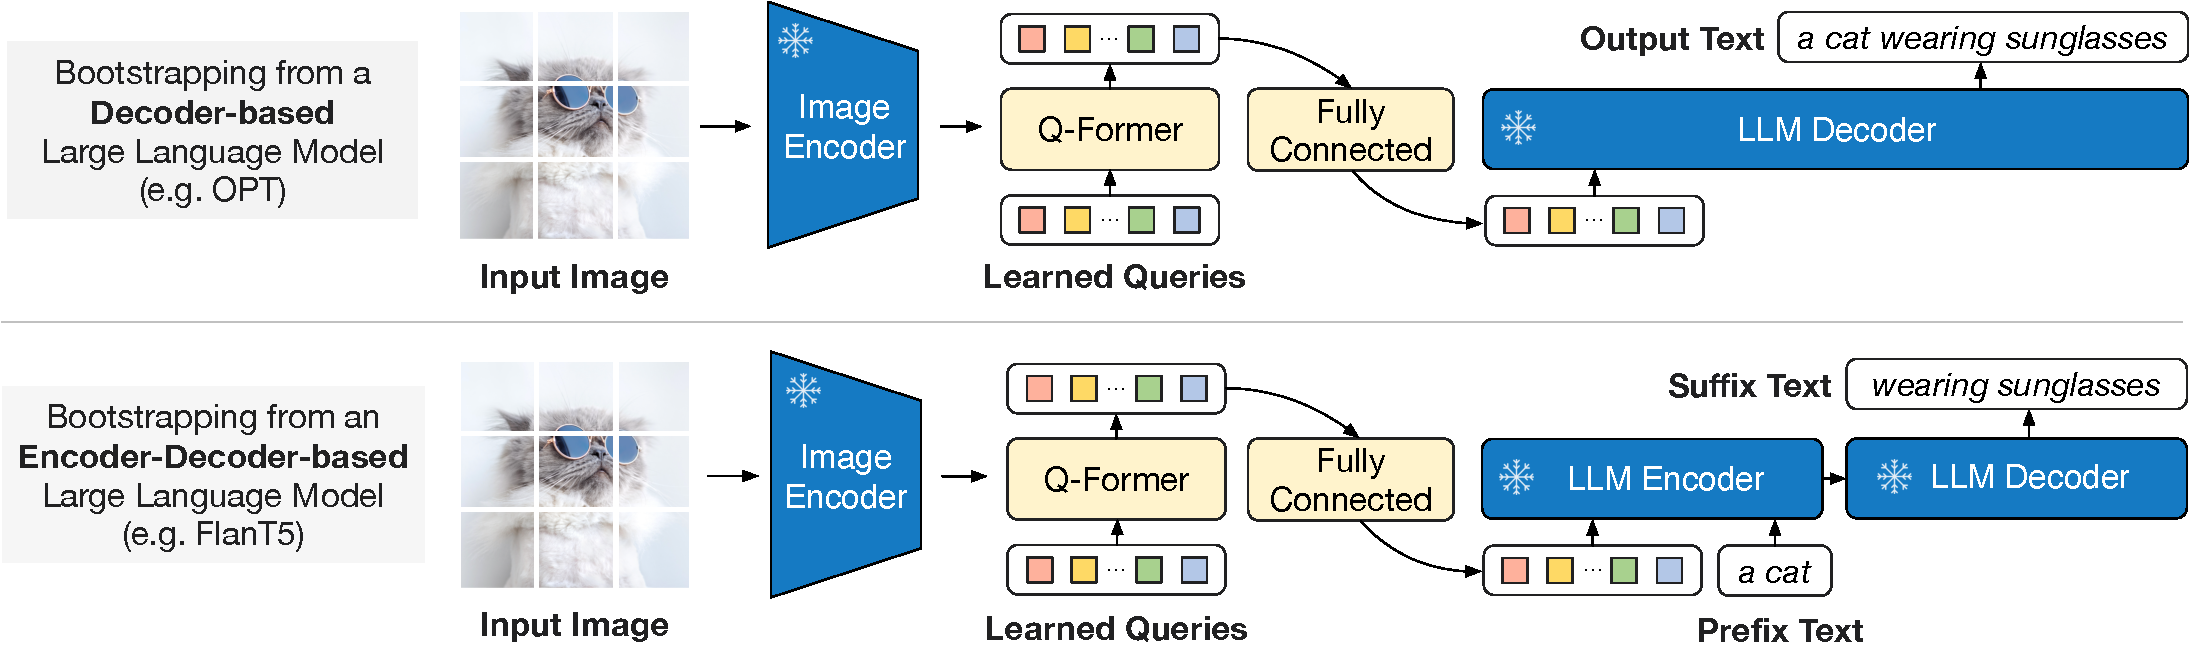
\includegraphics[width=0.9\textwidth]{image/fig3-v3.pdf}
\vspace{-2ex}
\caption{BLIP-2's second-stage vision-to-language generative pre-training, which bootstraps from frozen large language models (LLMs). (\textbf{Top}) Bootstrapping a decoder-based LLM (e.g. OPT). (\textbf{Bottom}) Bootstrapping an encoder-decoder-based LLM (e.g. FlanT5). The fully-connected layer adapts from the output dimension of the Q-Former to the input dimension of the chosen LLM.}
\vspace{-1.5ex}
\label{fig:stage2}
\end{figure*}

% \begin{figure*}[!t]
% \centering
% %   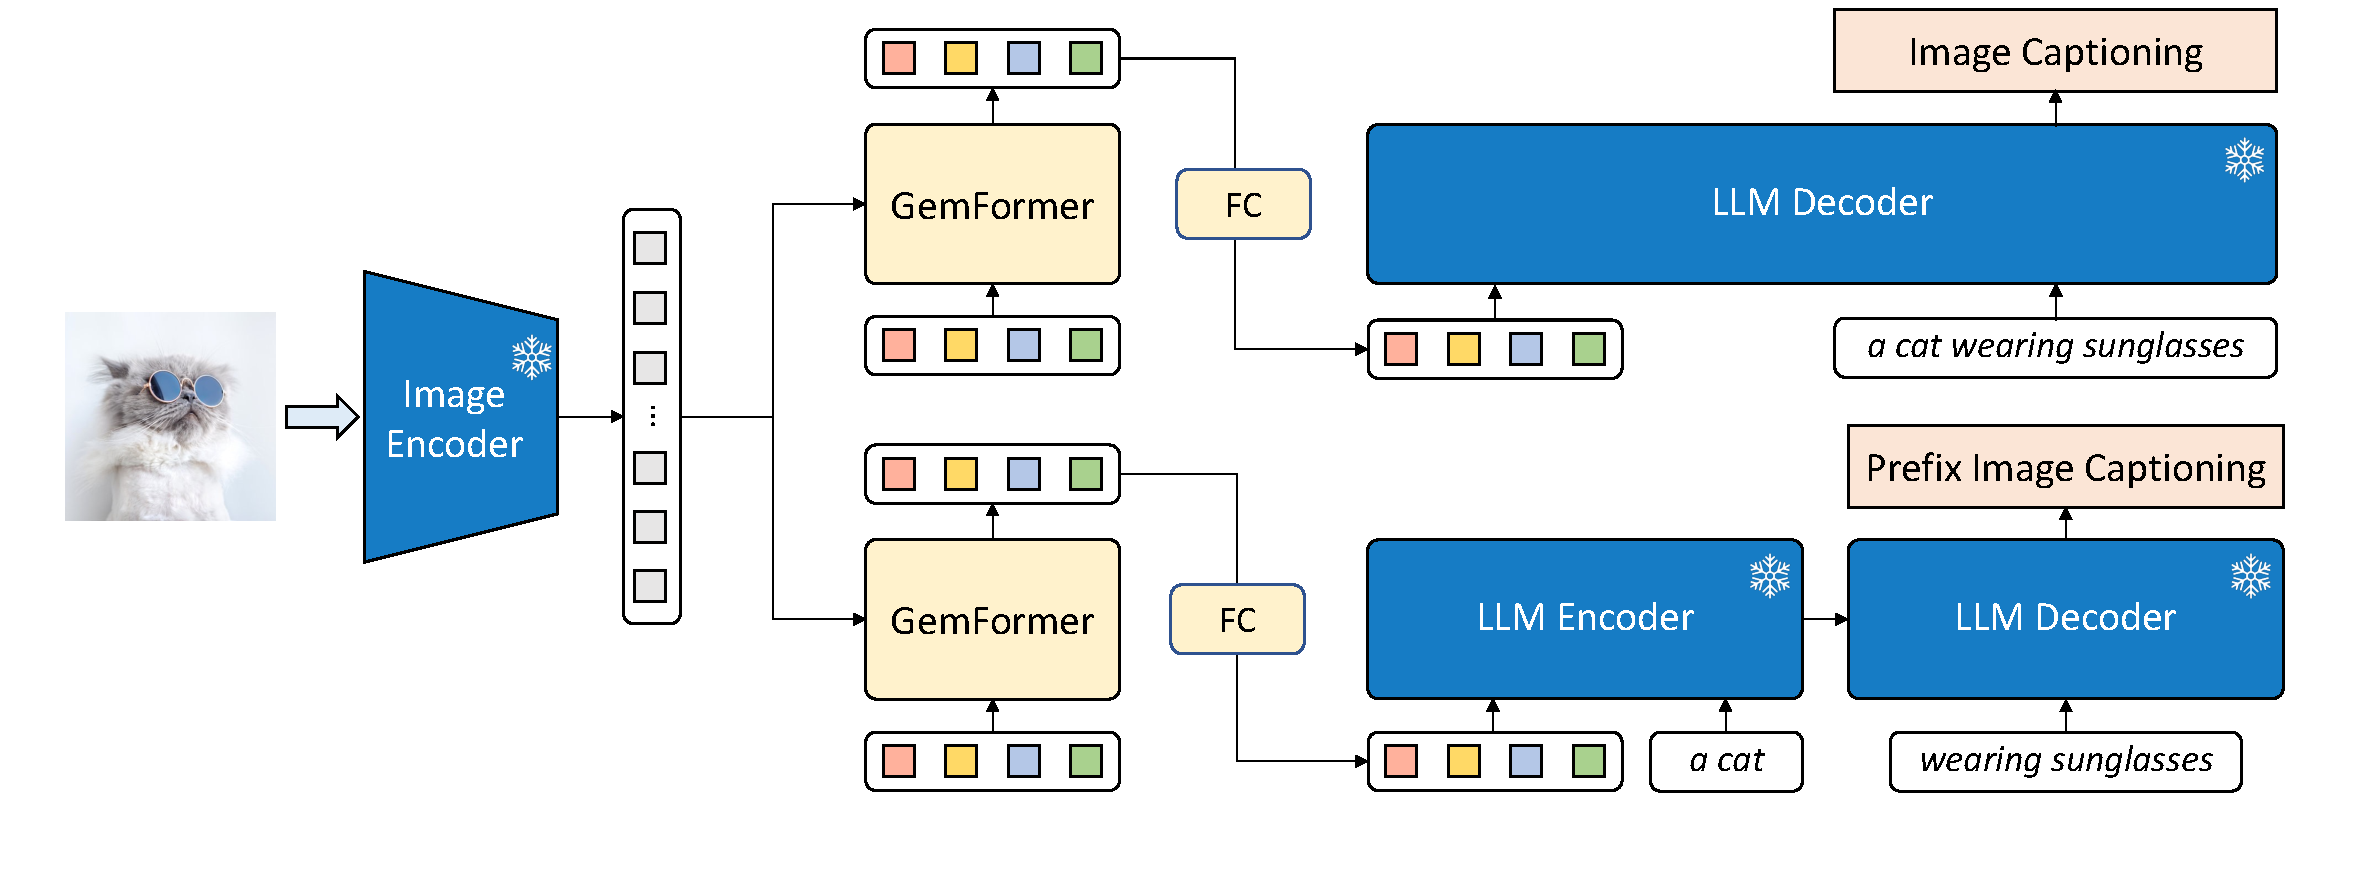
\includegraphics[width=\textwidth]{image/stage2.pdf}
%   
\includegraphics[width=0.8\textwidth]{BLIPv2/image/fig3-v2.pdf}
% \vspace{-2ex}
% \caption{Model architecture to bootstrap from frozen large language models (LLMs) with Q-Former. (\textbf{Top}) Bootstrapping a Decoder-based Large Language Model (e.g. OPT). (\textbf{Bottom}) Bootstrapping an Encoder-Decoder-based Large Language Model (e.g. FlanT5). The fully-connected layer adapts from the hidden dimension of the Q-Former to that of the chosen LLM.}
% %\vspace{-1ex}
% \label{fig:stage2}
% \end{figure*}



% \begin{figure*}[!t]
% \centering
% %   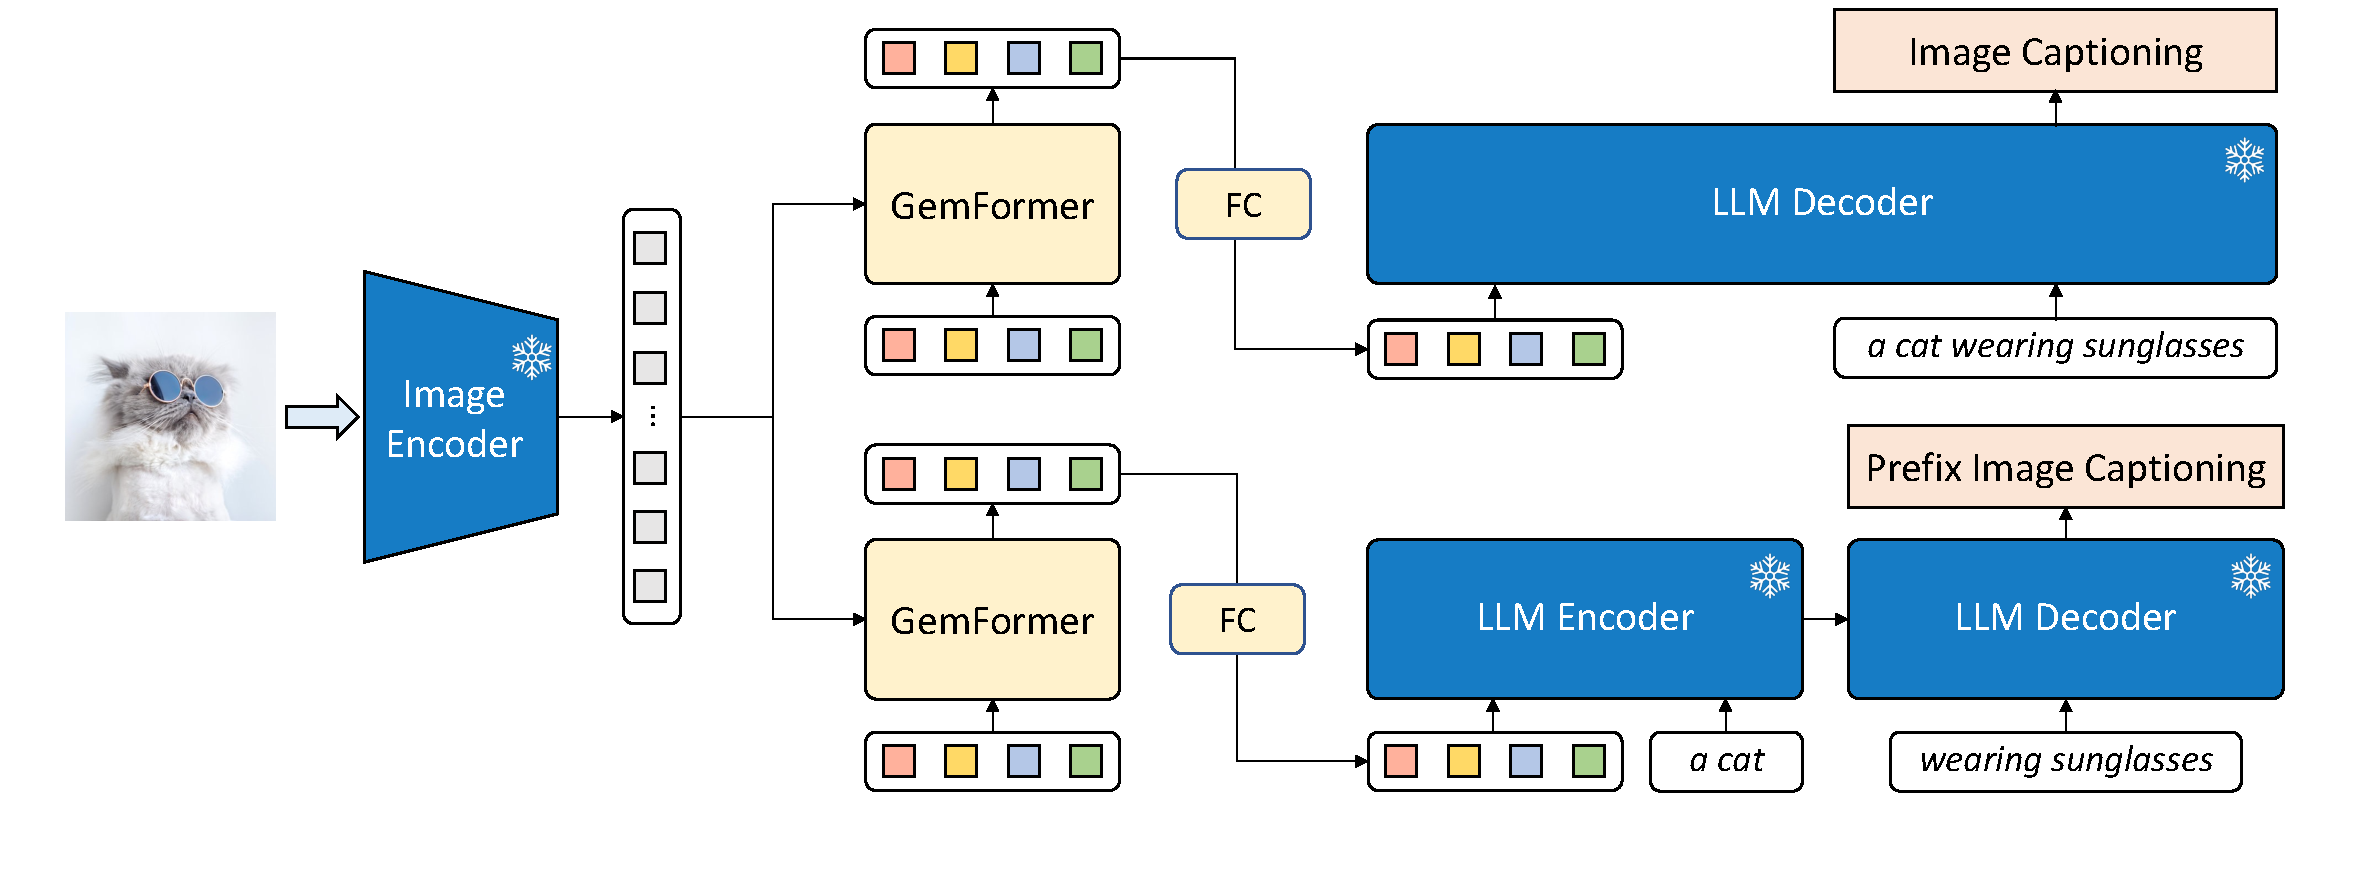
\includegraphics[width=\textwidth]{image/stage2.pdf}
%   
\includegraphics[width=0.8\textwidth]{BLIPv2/image/fig3-v2.pdf}
% \vspace{-2ex}
% \caption{Model architecture to bootstrap from frozen large language models (LLMs) with Q-Former. (\textbf{Top}) Bootstrapping a Decoder-based Large Language Model (e.g. OPT). (\textbf{Bottom}) Bootstrapping an Encoder-Decoder-based Large Language Model (e.g. FlanT5). The fully-connected layer adapts from hidden dimension in Q-Former to that of the chosen LLM.}
% %\vspace{-1ex}
% \label{fig:stage2}
% \end{figure*}


\vspace{-0.5ex}
\subsection{Bootstrap Vision-to-Language Generative Learning from a Frozen LLM}
\vspace{-0.5ex}
In the generative pre-training stage,
we connect \name~(with the frozen image encoder attached) to a frozen LLM to harvest the LLM's generative language capability.
As shown in Figure~\ref{fig:stage2},
we use a fully-connected (FC) layer to linearly project the output query embeddings $Z$ into the same dimension as the text embedding of the LLM. 
The projected query embeddings are then prepended to the input text embeddings.
They function as \textit{soft visual prompts} that condition the LLM on visual representation extracted by the \name.
Since the \name~has been pre-trained to extract language-informative visual representation,
it effectively functions as an information bottleneck that feeds the most useful information to the LLM while removing irrelevant visual information.
This reduces the burden of the LLM to learn vision-language alignment,
thus mitigating the catastrophic forgetting problem.
%~\cite{flamingo,Frozen}.


We experiment with two types of LLMs: decoder-based LLMs and encoder-decoder-based LLMs.
For decoder-based LLMs,
we pre-train with the language modeling loss,
where the frozen LLM is tasked to generate the text conditioned on the visual representation from \name.
For encoder-decoder-based LLMs,
we pre-train with the prefix language modeling loss,
where we split a text into two parts.
The prefix text is concatenated with the visual representation as input to the LLM's encoder.
The suffix text is used as the generation target for the LLM's decoder.

% \noindent\textbf{Image Captioning with Decoder LLM.}
% We pre-train with the image captioning loss when using a decoder LLM,
% where the frozen LLM is tasked to generate the text conditioned on the visual representation from \name.

% \noindent\textbf{Prefix Image Captioning with Encoder-Decoder LLM.}
% For an encoder-decoder LLM,
% we pre-train with the prefix image captioning task,
% where we split a caption into two parts.
% The first part is concatenated with the visual representation as input to the LLM's encoder.
% The second part is the generation target for the LLM's decoder.

% We also use \name~to modulate a direct information flow from the frozen image encoder to the LLM.   
% Specifically,
% for every $n$-th block in the LLM,
% each input query can attend to the image features through a cross-attention layer.
% The $K$ and $V$ of this attention layer are computed using frozen image features $I$.
% We linearly project the query embedding $Z$ and add it to the input for computing $Q$.
% Therefore, \name~controls the LLM's attention over the image features.
% We follow~\cite{flamingo} and multiply the cross-attention layer's output by tanh($\alpha$),
% where $\alpha$ is initialized at 0 to ensure a smooth injection of visual information into the language model.

% Different from the cross-attention layers in Flamingo~\cite{flamingo} where text tokens in the LLM can directly attend to the image,
% our cross-attention layers only apply to the queries.
% By decoupling image-text interaction into image-query and query-text information,
% we enable \name~to function as an information bottleneck that feeds the most useful visual information to the LLM.
% This architectural design minimally disrupts the original knowledge stored in the LLM, achieving fast vision-language alignment while mitigating catastrophic forgetting.

% During pre-training, we optimize the image captioning loss.


% We can further condition the \name~on text input for language-guided visual feature extraction.
% Depending on whether the downstream task has language input,
% we choose one of the following two pre-training objectives.

% \noindent\textbf{Prefix Image Captioning}
% randomly splits a text into two segments.
% The former segment is given as input to both the \name~and the language model.
% The later segment is used as the target to be generated by the language model.

% \noindent\textbf{Image Captioning}
% uses the entire text as the generation target.
% The \name~is not conditioned on any text.






\vspace{-0.5ex}
\subsection{Model Pre-training}
\vspace{-0.5ex}
\noindent\textbf{Pre-training data.}
We use the same pre-training dataset as BLIP with 129M images in total,
including COCO~\cite{coco}, Visual Genome~\cite{VG}, CC3M~\cite{CC}, CC12M~\cite{cc12m}, SBU~\cite{sbu}, and 115M images from the LAION400M dataset~\cite{laion}.
We adopt the CapFilt method~\cite{blip} to create synthetic captions for the web images.
Specifically, we generate 10 captions using the BLIP$_\mathrm{large}$ captioning model, and rank the synthetic captions along with the original web caption based on the image-text similarity produced by a CLIP ViT-L/14 model.
% \DX{we can be more specific with which CLIP model is used. Also, we have a preference score 0.2 added to the original caption. Not sure should we mention this or not.}.
We keep top-two captions per image as training data and randomly sample one at each pre-training step.


\noindent\textbf{Pre-trained image encoder and LLM.}
For the frozen image encoder, we explore two state-of-the-art pre-trained vision transformer models: (1) ViT-L/14 from CLIP~\cite{clip} and (2) ViT-g/14 from EVA-CLIP~\cite{eva}.
We remove the last layer of the ViT and uses the second last layer's output features,
which leads to slightly better performance.
For the frozen language model,
we explore the unsupervised-trained OPT model family~\cite{opt} for decoder-based LLMs,
and the instruction-trained FlanT5 model family~\cite{flanT5} for encoder-decoder-based LLMs.


\begin{figure*}[!t]
\centering
  
\includegraphics[width=\textwidth]{image/examples}
\vspace{-15ex}
\caption{Selected examples of \textbf{instructed zero-shot image-to-text generation} using a BLIP-2 model w/ ViT-g and FlanT5$_\text{XXL}$,
where it shows a wide range of capabilities including
visual conversation, visual knowledge reasoning, visual commensense reasoning,
storytelling, personalized image-to-text generation, etc.
}
%\vspace{-1ex}
\label{fig:example}
\end{figure*}


\noindent\textbf{Pre-training settings.}
We pre-train for 250k steps in the first stage and 80k steps in the second stage.
We use a batch size of 2320/1680 for ViT-L/ViT-g in the first stage and a batch size of 1920/1520 for OPT/FlanT5 in the second stage.
During pre-training, we convert the frozen ViTs' and LLMs' parameters into FP16, except for FlanT5 where we use BFloat16.
We found no performance degradation compared to using 32-bit models.
Due to the use of frozen models,
our pre-training is more computational friendly than existing large-scale VLP methods.
For example,
using a single 16-A100(40G) machine,
our largest model with ViT-g and FlanT5-XXL requires less than 6 days for the first stage and less than 3 days for the second stage.

The same set of pre-training hyper-parameters are used for all models.
We use the AdamW~\cite{adamw} optimizer with $\beta_1=0.9$, $\beta_1=0.98$, and a weight decay of 0.05.
We use a cosine learning rate decay with a peak learning rate of 1e-4 and a linear warmup of 2k steps. 
The minimum learning rate at the second stage is 5e-5.
We use images of size 224$\times$224, augmented with random resized cropping and horizontal flipping.








